\documentclass{standalone}
\usepackage{tikz}
\usetikzlibrary{patterns, positioning}
\usepackage[sfdefault]{ClearSans} %% option 'sfdefault' activates Clear Sans as the default text font
\usepackage[T1]{fontenc}

\begin{document}
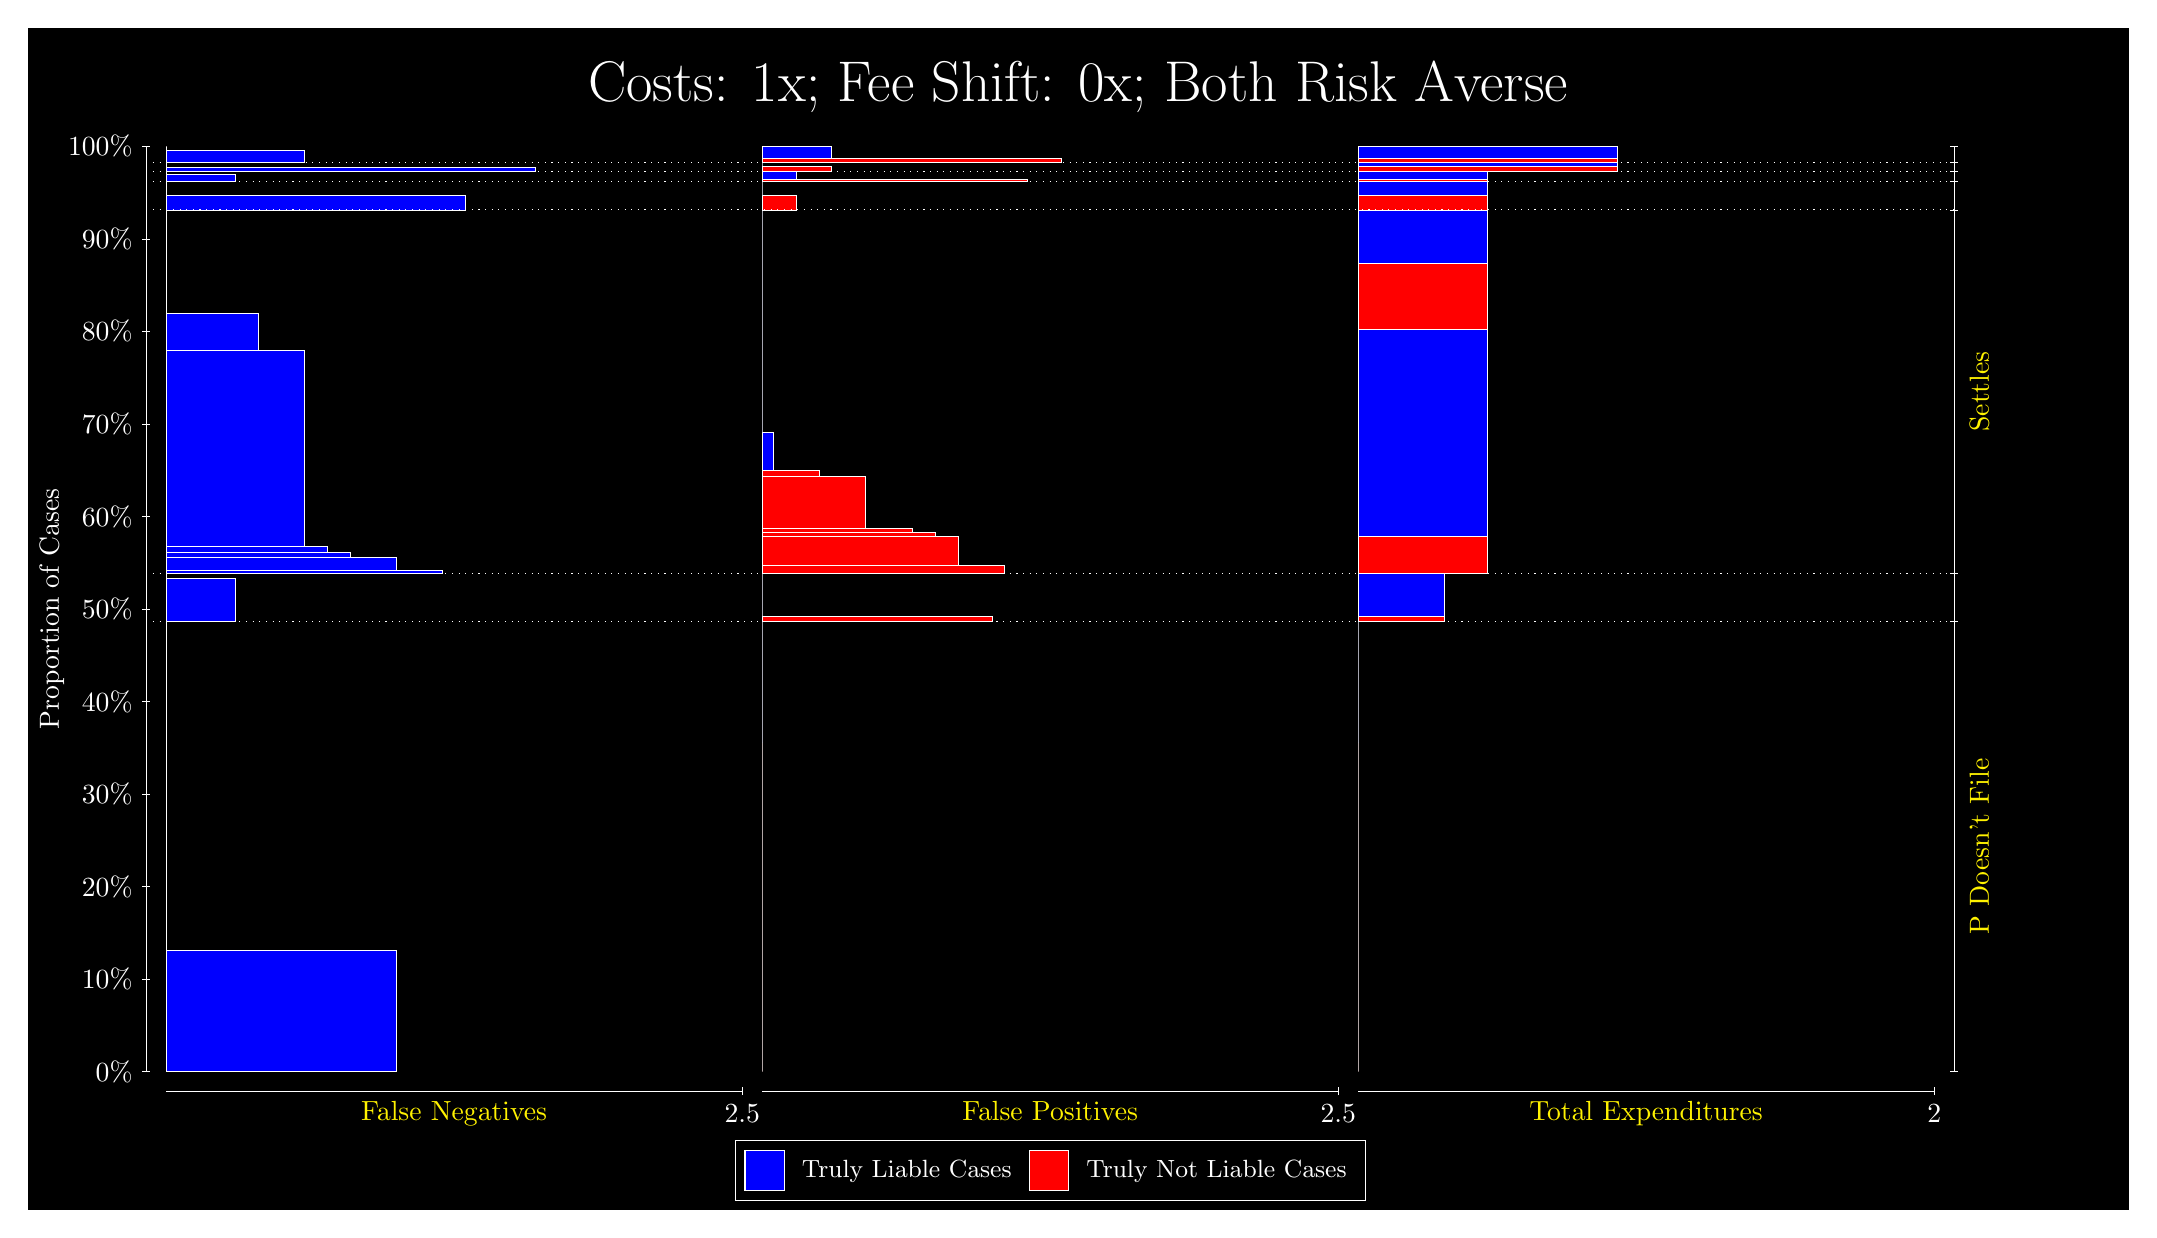
\begin{tikzpicture}
\draw[fill=black] (0,0) rectangle (26.667,15);
\draw[text=white] (0,13.5) rectangle (26.667,15) node[midway] {\huge Costs: 1x; Fee Shift: 0x; Both Risk Averse};
\draw[white, very thin] (1.5,1.75) -- (1.5,13.5);
\node[rotate=90, text=white, anchor=center] at (0.3, 7.625) {Proportion of Cases};
\draw[white, very thin] (1.45,1.75) -- (1.55,1.75);
\node[text=white, anchor=east] at (1.45, 1.75) {0\%};
\draw[white, very thin] (1.45,2.925) -- (1.55,2.925);
\node[text=white, anchor=east] at (1.45, 2.925) {10\%};
\draw[white, very thin] (1.45,4.1) -- (1.55,4.1);
\node[text=white, anchor=east] at (1.45, 4.1) {20\%};
\draw[white, very thin] (1.45,5.275) -- (1.55,5.275);
\node[text=white, anchor=east] at (1.45, 5.275) {30\%};
\draw[white, very thin] (1.45,6.45) -- (1.55,6.45);
\node[text=white, anchor=east] at (1.45, 6.45) {40\%};
\draw[white, very thin] (1.45,7.625) -- (1.55,7.625);
\node[text=white, anchor=east] at (1.45, 7.625) {50\%};
\draw[white, very thin] (1.45,8.8) -- (1.55,8.8);
\node[text=white, anchor=east] at (1.45, 8.8) {60\%};
\draw[white, very thin] (1.45,9.975) -- (1.55,9.975);
\node[text=white, anchor=east] at (1.45, 9.975) {70\%};
\draw[white, very thin] (1.45,11.15) -- (1.55,11.15);
\node[text=white, anchor=east] at (1.45, 11.15) {80\%};
\draw[white, very thin] (1.45,12.325) -- (1.55,12.325);
\node[text=white, anchor=east] at (1.45, 12.325) {90\%};
\draw[white, very thin] (1.45,13.5) -- (1.55,13.5);
\node[text=white, anchor=east] at (1.45, 13.5) {100\%};

\draw[white, very thin] (24.457,1.75) -- (24.457,13.5);
\draw[white, very thin] (24.407,1.75) -- (24.507,1.75);
\node[anchor=west] at (24.407, 1.75) {};
\draw[white, very thin] (24.407,7.4676) -- (24.507,7.4676);
\node[anchor=west] at (24.407, 7.4676) {};
\draw[white, very thin] (24.407,8.0776) -- (24.507,8.0776);
\node[anchor=west] at (24.407, 8.0776) {};
\draw[white, very thin] (24.407,12.694) -- (24.507,12.694);
\node[anchor=west] at (24.407, 12.694) {};
\draw[white, very thin] (24.407,13.054) -- (24.507,13.054);
\node[anchor=west] at (24.407, 13.054) {};
\draw[white, very thin] (24.407,13.179) -- (24.507,13.179);
\node[anchor=west] at (24.407, 13.179) {};
\draw[white, very thin] (24.407,13.297) -- (24.507,13.297);
\node[anchor=west] at (24.407, 13.297) {};
\draw[white, very thin] (24.407,13.5) -- (24.507,13.5);
\node[anchor=west] at (24.407, 13.5) {};

\draw[white, very thin, fill=blue] (1.75,1.75) rectangle (4.6775,3.293);
\draw[white, very thin, fill=red] (1.75,3.293) rectangle (1.75,7.4676);
\draw[white, very thin, fill=blue] (1.75,7.4676) rectangle (2.6283,8.0169);
\draw[white, very thin, fill=red] (1.75,8.0169) rectangle (1.75,8.0776);
\draw[white, very thin, fill=blue] (1.75,8.0776) rectangle (5.2631,8.1139);
\draw[white, very thin, fill=blue] (1.75,8.1139) rectangle (4.6775,8.2755);
\draw[white, very thin, fill=blue] (1.75,8.2755) rectangle (4.092,8.3397);
\draw[white, very thin, fill=blue] (1.75,8.3397) rectangle (3.7993,8.4152);
\draw[white, very thin, fill=blue] (1.75,8.4152) rectangle (3.5065,10.906);
\draw[white, very thin, fill=blue] (1.75,10.906) rectangle (2.921,11.385);
\draw[white, very thin, fill=red] (1.75,11.385) rectangle (1.75,12.694);
\draw[white, very thin, fill=blue] (1.75,12.694) rectangle (5.5558,12.874);
\draw[white, very thin, fill=red] (1.75,12.874) rectangle (1.75,13.054);
\draw[white, very thin, fill=blue] (1.75,13.054) rectangle (2.6283,13.146);
\draw[white, very thin, fill=red] (1.75,13.146) rectangle (1.75,13.179);
\draw[white, very thin, fill=blue] (1.75,13.179) rectangle (6.4341,13.229);
\draw[white, very thin, fill=red] (1.75,13.229) rectangle (1.75,13.297);
\draw[white, very thin, fill=blue] (1.75,13.297) rectangle (3.5065,13.449);
\draw[white, very thin, fill=red] (1.75,13.449) rectangle (1.75,13.5);
\draw[white, very thin, fill=red] (9.3189,1.75) rectangle (9.3189,5.9246);
\draw[white, very thin, fill=blue] (9.3189,5.9246) rectangle (9.3189,7.4676);
\draw[white, very thin, fill=red] (9.3189,7.4676) rectangle (12.246,7.5283);
\draw[white, very thin, fill=blue] (9.3189,7.5283) rectangle (9.3189,8.0776);
\draw[white, very thin, fill=red] (9.3189,8.0776) rectangle (12.393,8.1751);
\draw[white, very thin, fill=red] (9.3189,8.1751) rectangle (11.807,8.5512);
\draw[white, very thin, fill=red] (9.3189,8.5512) rectangle (11.515,8.602);
\draw[white, very thin, fill=red] (9.3189,8.602) rectangle (11.222,8.6438);
\draw[white, very thin, fill=red] (9.3189,8.6438) rectangle (10.636,9.3041);
\draw[white, very thin, fill=red] (9.3189,9.3041) rectangle (10.051,9.3863);
\draw[white, very thin, fill=blue] (9.3189,9.3863) rectangle (9.4652,9.8655);
\draw[white, very thin, fill=blue] (9.3189,9.8655) rectangle (9.3189,12.694);
\draw[white, very thin, fill=red] (9.3189,12.694) rectangle (9.758,12.874);
\draw[white, very thin, fill=blue] (9.3189,12.874) rectangle (9.3189,13.054);
\draw[white, very thin, fill=red] (9.3189,13.054) rectangle (12.686,13.086);
\draw[white, very thin, fill=blue] (9.3189,13.086) rectangle (9.758,13.179);
\draw[white, very thin, fill=red] (9.3189,13.179) rectangle (10.197,13.247);
\draw[white, very thin, fill=blue] (9.3189,13.247) rectangle (9.3189,13.297);
\draw[white, very thin, fill=red] (9.3189,13.297) rectangle (13.125,13.348);
\draw[white, very thin, fill=blue] (9.3189,13.348) rectangle (10.197,13.5);
\draw[white, very thin, fill=red] (16.888,1.75) rectangle (16.888,5.9246);
\draw[white, very thin, fill=blue] (16.888,5.9246) rectangle (16.888,7.4676);
\draw[white, very thin, fill=red] (16.888,7.4676) rectangle (17.986,7.5283);
\draw[white, very thin, fill=blue] (16.888,7.5283) rectangle (17.986,8.0776);
\draw[white, very thin, fill=red] (16.888,8.0776) rectangle (18.534,8.5463);
\draw[white, very thin, fill=blue] (16.888,8.5463) rectangle (18.534,11.177);
\draw[white, very thin, fill=red] (16.888,11.177) rectangle (18.534,12.017);
\draw[white, very thin, fill=blue] (16.888,12.017) rectangle (18.534,12.694);
\draw[white, very thin, fill=red] (16.888,12.694) rectangle (18.534,12.874);
\draw[white, very thin, fill=blue] (16.888,12.874) rectangle (18.534,13.054);
\draw[white, very thin, fill=red] (16.888,13.054) rectangle (18.534,13.086);
\draw[white, very thin, fill=blue] (16.888,13.086) rectangle (18.534,13.179);
\draw[white, very thin, fill=red] (16.888,13.179) rectangle (20.181,13.247);
\draw[white, very thin, fill=blue] (16.888,13.247) rectangle (20.181,13.297);
\draw[white, very thin, fill=red] (16.888,13.297) rectangle (20.181,13.348);
\draw[white, very thin, fill=blue] (16.888,13.348) rectangle (20.181,13.5);
\draw[white, dotted] (1.5,7.4676) -- (24.457,7.4676);
\draw[white, dotted] (1.5,8.0776) -- (24.457,8.0776);
\draw[white, dotted] (1.5,12.694) -- (24.457,12.694);
\draw[white, dotted] (1.5,13.054) -- (24.457,13.054);
\draw[white, dotted] (1.5,13.179) -- (24.457,13.179);
\draw[white, dotted] (1.5,13.297) -- (24.457,13.297);
\draw[white, very thin] (1.75,1.5) -- (9.0689,1.5);
\node[text=yellow, anchor=north] at (5.4094, 1.5) {False Negatives};
\draw[white, very thin] (9.0689,1.45) -- (9.0689,1.55);
\node[text=white, anchor=north] at (9.0689, 1.45) {2.5};

\draw[white, very thin] (9.3189,1.5) -- (16.638,1.5);
\node[text=yellow, anchor=north] at (12.978, 1.5) {False Positives};
\draw[white, very thin] (16.638,1.45) -- (16.638,1.55);
\node[text=white, anchor=north] at (16.638, 1.45) {2.5};

\draw[white, very thin] (16.888,1.5) -- (24.207,1.5);
\node[text=yellow, anchor=north] at (20.547, 1.5) {Total Expenditures};
\draw[white, very thin] (24.207,1.45) -- (24.207,1.55);
\node[text=white, anchor=north] at (24.207, 1.45) {2};

\node[text=yellow, centered, rotate=90] at (24.777, 4.6088) {P Doesn't File};

\node[text=yellow, centered, rotate=90] at (24.777, 10.386) {Settles};





\draw (12.978300999999998,1.5) node[draw=none] (baseCoordinate) {};
\begin{scope}[align=center]
        \matrix[scale=0.5, draw=white, below=0.5cm of baseCoordinate, nodes={draw}, column sep=0.1cm]{
            \node[rectangle, draw, minimum width=0.5cm, minimum height=0.5cm, fill=blue] {}; &
            \node[draw=none, font=\small, text=white] (B) {Truly Liable Cases}; &
            \node[rectangle, draw, minimum width=0.5cm, minimum height=0.5cm, fill=red] {}; &
            \node[draw=none, font=\small, text=white] (B) {Truly Not Liable Cases}; \\
            };
\end{scope}

\end{tikzpicture}
\end{document}